%%%%%%%%%%%%%%%%%%%%%%%%%%%%%%%%%%%%%%%%%%%%%%%%%%%%
\documentclass[fleqn,10pt,twocolumn]{SICE_FES25}

\usepackage{amsmath}
\usepackage{amssymb}
\let\proof\relax
\let\endproof\relax
\usepackage{amsthm}

\theoremstyle{definition}
\newtheorem{definition}{Definition}
\theoremstyle{plain}
\newtheorem{mytheorem}{Theorem}

\title{Feature-Driven Field-of-View Overlap Assurance with CBFs \\ for Cooperative Visual Localization}

\author{Tomoki Arita${}^{1\dagger}$ and Toru Namerikawa${}^{2}$}
% The dagger symbol indicates the presenter.
\speaker{Tomoki Arita}

\affils{${}^{1}$School of Integrated Design Engineering, Keio University, Kanagawa, Japan\\
${}^{2}$Department of System Design Engineering, Keio University, Kanagawa, Japan\\
(Tel: +81-45-563-1151; E-mail: arita.tomoki@keio.jp, namerikawa@sd.keio.ac.jp)\\
}
\abstract{%
This paper proposes a distributed control barrier functions (CBFs) approach to guarantee field-of-view overlap for cooperative visual localization in multi-agent systems. We formulate the problem on the Special Euclidean Group SE(3) and introduce a probabilistic CBFs that evaluates the visibility of feature points to ensure that multiple agents maintain shared visual features. The proposed method incorporates a distributed optimization algorithm based on the primal-dual method of multipliers (PDMM), enabling each agent to compute control inputs locally while satisfying global safety constraints. Simulation results demonstrate the effectiveness of our approach in both centralized and distributed implementations, showing that agents can maintain shared field-of-view while following desired trajectories.
}

\keywords{%
Control barrier function, Multi-agent systems, Cooperative localization, Field-of-view constraints, Distributed optimization
}

\begin{document}

\maketitle

%-----------------------------------------------------------------------

\section{Introduction}

In multi-agent systems, sharing sensor information and visual field among agents enables efficient execution of tasks such as surveillance, search, and cooperative transportation. Particularly in visual cooperation using cameras, a common field-of-view (CoFoV) among agents is essential. For example, multiple drones need to observe the same target from different angles, or maintain line-of-sight (LOS) communication \cite{ref1}.

In multi-agent Visual Simultaneous Localization and Mapping (VSLAM), each agent performs self-localization based on local features extracted from captured images, and estimates relative positions through feature matching between agents. Learning-based local feature detectors and descriptors such as SuperPoint \cite{ref2}, which have replaced traditional ORB and SIFT, and global descriptors like NetVLAD \cite{ref3}, have shown high robustness, contributing to loop detection and keyframe matching.

For successful matching of image features, geometric overlap of camera view frustums is necessary to ensure that agents observe common landmarks. When view overlap exists, loop detection between agents becomes possible, enabling map integration among robots \cite{ref4}. However, since robots have limited field-of-view angles, developing control techniques to guarantee shared view is urgent.

\begin{figure}[ht]
\begin{center}
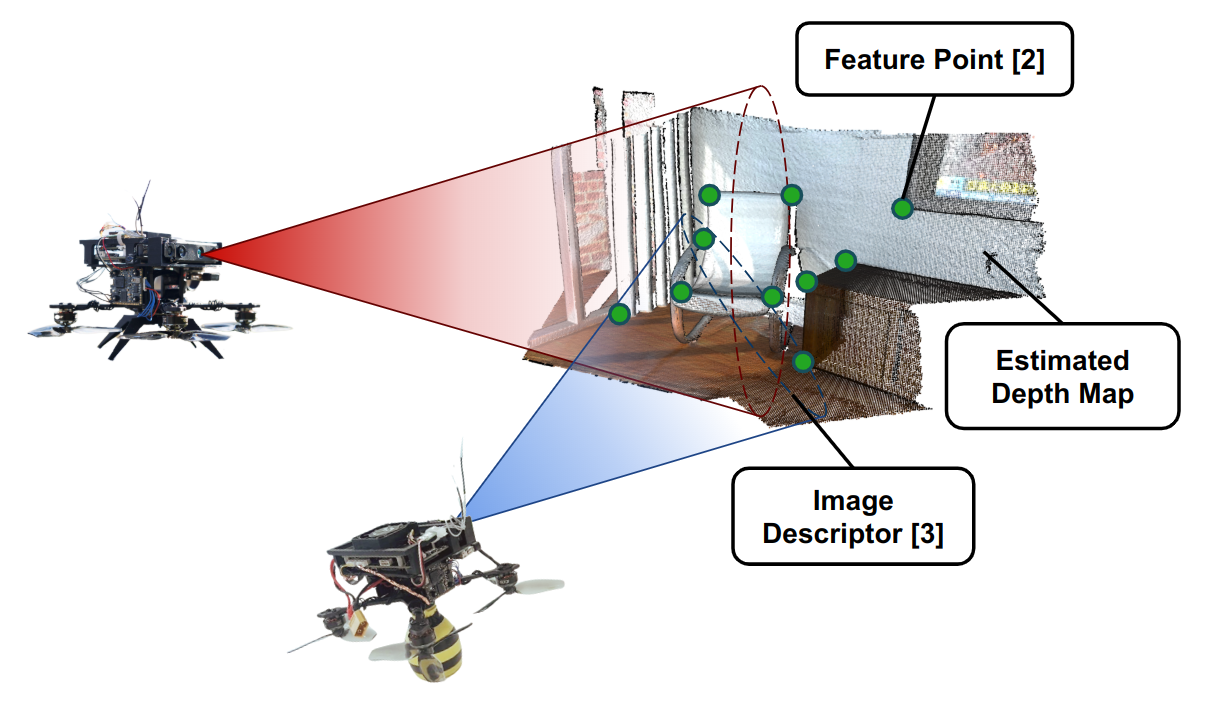
\includegraphics[width=8cm]{Fig/covins_system.eps}
\caption{\label{fig:covins} Architecture of cooperative visual-inertial SLAM using visual features and descriptors.}
\vspace{-6mm}
\end{center}
\end{figure}

\subsection{Related Work}

Previous approaches have used potential fields or Model Predictive Control (MPC) to address formation control and sensor graph connectivity maintenance under local visibility constraints \cite{ref5}. Meanwhile, CBFs have emerged as promising candidates as they can compute optimal control inputs in real-time while preventing constraint violations \cite{ref6} \cite{ref7}.

However, current cooperative SLAM systems rely on passive sharing of keyframes and image similarity evaluation, risking failure in map integration if view overlap does not occur incidentally. Furthermore, centralized control becomes impractical for large numbers of robots due to communication load and computational complexity, necessitating distributed algorithms where each agent computes locally and coordinates with limited communication.

Traditional view maintenance methods have typically evaluated target visibility deterministically, without adequately incorporating sensor observation uncertainties \cite{ref8}. Additionally, many view-constrained control methods have been based on simplified dynamic models (e.g., Dubins vehicles or quadrotors with horizontal attitude maintenance), without explicitly considering rigid-body dynamics \cite{ref9}.

\subsection{Contributions}

This paper proposes a distributed CBFs approach to guarantee field-of-view overlap for cooperative localization on SE(3). Our main contributions are:

\begin{itemize}
\item We achieve field-of-view guarantee on SE(3).~While conventional stereo vision or leader-follower approaches merely constrain relative geometric configurations between robots, our framework provides integrated control of position and attitude for all agents in three-dimensional space.
\item We apply probabilistic visibility constraints based on feature points to CBFs.~Our approach probabilistically evaluates the visibility of feature points observed by each agent and incorporates this into CBFs, designing control inputs to ensure high probability of shared view maintenance.~This enables safe view maintenance even under uncertainty from sensor noise.
\item We implement distributed optimization for rigid-body dynamics.~Our approach introduces CBFs to handle rigid-body drone models on SE(3) that consider both translational and rotational motion simultaneously, and proposes a framework where each agent computes control solutions through distributed optimization algorithms (e.g., PDMM) via local information exchange.~This achieves both real-time performance and scalability.
\end{itemize}

\section{Preliminary: Control Barrier Function}

This section introduces the basic concept of CBF\cite{ref6}, which form the foundation of our approach.

Consider a continuous-time control-affine system:
\begin{equation}
\begin{aligned}
\dot{{\mathbf{x}}} = f({\mathbf{x}}) + g({\mathbf{x}}){\mathbf{u}}
\label{eq:control_affine}
\end{aligned}
\end{equation}
where ${\mathbf{x}}(t) \in {\mathbb{B}}^n$ is the state, ${\mathbf{u}}(t) \in {\mathbb{R}}^m$ is the control input, and $f: {\mathbb{R}}^n \rightarrow {\mathbb{R}}^n$ and $g: {\mathbb{R}}^n \rightarrow {\mathbb{R}}^{n \times m}$ are locally Lipschitz continuous functions.

We define a safe set ${\mathcal{C}}$ as:
\begin{equation}
\begin{aligned}
{\mathcal{C}} = \{{\mathbf{x}} \in {\mathbb{R}}^n : h({\mathbf{x}}) \geq 0\}
\label{eq:safe_set}
\end{aligned}
\end{equation}
where $h: {\mathbb{R}}^n \rightarrow {\mathbb{R}}$ is a continuously differentiable function.

\begin{definition}[Control Barrier Function\cite{ref6}]
A continuously differentiable function $h: {\mathbb{R}}^n \rightarrow {\mathbb{R}}$ with non-vanishing gradient $\nabla h({\mathbf{x}})$ on ${\mathcal{C}}$ is a control barrier function if there exists an extended class $\mathcal{K}_{\infty}$ function $\alpha$ such that for any ${\mathbf{x}} \in {\mathcal{C}}$, there exists a control input ${\mathbf{u}} \in {\mathbb{R}}^m$ satisfying:
\begin{equation}
\begin{aligned}
L_f h({\mathbf{x}}) + L_g h({\mathbf{x}}){\mathbf{u}} + \alpha(h({\mathbf{x}})) \geq 0
\label{eq:cbf_condition}
\end{aligned}
\end{equation}
where $L_f h({\mathbf{x}}) = \nabla h({\mathbf{x}})^T f({\mathbf{x}})$ and $L_g h({\mathbf{x}}) = \nabla h({\mathbf{x}})^T g({\mathbf{x}})$ are the Lie derivatives of $h$ with respect to $f$ and $g$, respectively.
\end{definition}

An important property of CBF is that any control input ${\mathbf{u}}$ satisfying \eqref{eq:cbf_condition} renders the safe set ${\mathcal{C}}$ forward invariant. That is, if the initial state ${\mathbf{x}}(0) \in {\mathcal{C}}$, then ${\mathbf{x}}(t) \in {\mathcal{C}}$ for all $t \geq 0$.

In practical control design, we often seek an optimal control input that satisfies the CBF constraint while achieving control objectives. This can be formulated as a Quadratic Programming (QP) problem:
\begin{equation}
\begin{aligned}
{\mathbf{u}}^* &= \underset{{\mathbf{u}} \in {\mathbb{R}}^m}{\text{arg min}} \:\: \|{\mathbf{u}} - {\mathbf{u}}_{\text{nom}}\|^2 \\
\text{s.t.} & \:\: L_f h({\mathbf{x}}) + L_g h({\mathbf{x}}){\mathbf{u}} + \alpha(h({\mathbf{x}})) \geq 0
\label{eq:cbf_qp}
\end{aligned}
\end{equation}
where ${\mathbf{u}}_{\text{nom}}$ is the nominal control input without considering safety constraints.

\section{Problem Formulation}

This section describes the system model, the definition of shared field-of-view, and the problem formulation.

\subsection{System Model: Rigid Body Motion on SE(3)}

We consider multiple drones moving on SE(3). The position and attitude of each agent $i \in \mathcal{A}$ are represented by an element $T_i = (p_i, R_i) \in \mathrm{SE}(3)$, where $p_i(t) \in {\mathbb{R}}^3$ is the position vector and $R_i(t) \in \mathrm{SO}(3)$ is the rotation matrix.

Rigid body motion on SE(3) can be described using the matrix representation:
\begin{equation}
\begin{aligned}
T_i &= \begin{bmatrix}
R_i & p_i \\
0 & 1
\end{bmatrix} \in \mathrm{SE}(3)
\label{eq:se3_matrix}
\end{aligned}
\end{equation}

The rigid body motion equation on SE(3) with body velocity input $\xi^\wedge_{B,i}$ is given by
\begin{equation}
\begin{aligned}
\dot{T}_i &= T_i \xi^\wedge_{B,i} \\
\xi^\wedge_{B,i} &= \begin{bmatrix}
[\omega_i]_\times & v_{i} \\
0 & 0
\end{bmatrix} \in \mathfrak{se}(3)
\label{eq:se3_dynamics_body}
\end{aligned}
\end{equation}
where $\omega_i \in {\mathbb{R}}^3$ is the angular velocity vector, $v_{i} \in {\mathbb{R}}^3$ is the translational velocity vector in the body frame, and $[\cdot]_\times: {\mathbb{R}}^3 \rightarrow \mathfrak{so}(3)$ is the skew-symmetric matrix operator.

In the world frame, the simplified dynamics can be written as
\begin{equation}
\begin{aligned}
\dot{R}_i &= R_i[\omega_i]_\times \\
\dot{p}_i &= R_i v_i
\label{eq:se3_dynamics_simplified}
\end{aligned}
\end{equation}
% where $v_i = R_iv_{B,i}$ is the translational velocity in the world frame.

\subsection{Field-of-View Definition}

Let $q_l \in \mathcal{L}$ be a feature point in the environment, and ${\mathcal{C}}_i$ be the set of feature points observed by agent $i$. The condition for a feature point $q_l$ to be within the field-of-view of agent $i$ is defined as:
\begin{equation}
\begin{aligned}
q_l \in {\mathcal{C}}_i \iff \beta_l^{\top}(p_i)R_ie_c - \cos\Psi_{\mathcal{F}} > 0
\label{eq:fov_condition}
\end{aligned}
\end{equation}
where $\beta_l(p_i) = \frac{q_l-p_i}{\|q_l-p_i\|}$ is the unit direction vector from agent $i$ to feature point $q_l$, $e_c$ is the unit vector representing the camera direction, and $\Psi_{\mathcal{F}}$ is the field-of-view angle.

The condition for multiple agents to observe a common feature point (shared field-of-view condition) is defined as:
\begin{equation}
\begin{aligned}
&q_l \in {{\mathcal{C}}}_i \cap {{\mathcal{C}}}_j \\
&\iff \beta_l^{\top}(p_i)R_ie_c - \cos\Psi_{\mathcal{F}} > 0 \\
&\:\:\:\qquad \text{ and } \beta_l^{\top}(p_j)R_je_c - \cos\Psi_{\mathcal{F}} > 0
\label{eq:shared_fov_condition}
\end{aligned}
\end{equation}
This condition means that the feature point $q_l$ is within the field-of-view of both agents.

\begin{figure}[ht]
\begin{center}
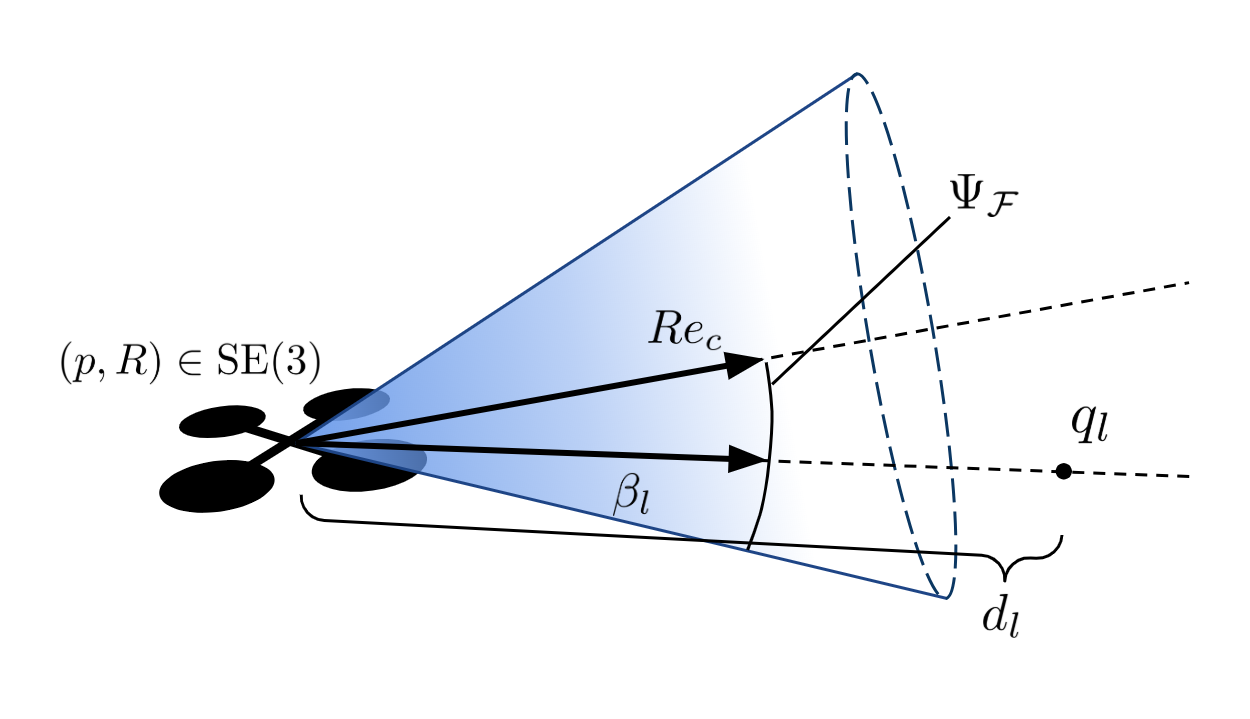
\includegraphics[width=7.5cm]{Fig/geometry.eps}
\caption{\label{fig:geometry} Geometric conditions for feature point observation.}
\vspace{-6mm}
\end{center}
\end{figure}

\subsection{Problem Statement}

The objective of this research is to design control inputs for multiple agents to ensure they always observe common feature points. Specifically, we consider the following problem:

\begin{definition}[Field-of-View Guarantee Problem]
Given a set of agents $\mathcal{A}$ and a set of feature points $\mathcal{L}$, design control inputs $\xi_{B,i} = (\omega_i, v_{B,i})$ for each agent $i \in \mathcal{A}$ such that:
\begin{enumerate}
\item Each agent $i$ moves toward its desired position $p_i^d$.
\item Between each pair of agents $i$ and $j$, at least $m$ common feature points are always observable, i.e., $|{\mathcal{C}}_i \cap {\mathcal{C}}_j| \geq m$ holds at all times.
\end{enumerate}
\end{definition}

To address this problem, we propose a CBF-based approach. In particular, we probabilistically evaluate feature point visibility and incorporate it into CBF to achieve safe field-of-view sharing even under uncertainty. We also develop a distributed optimization framework where each agent computes control inputs locally.

\section{CBF For Field-of-View Overlap}

This section presents the design of CBF to guarantee field-of-view overlap. We first derive safety constraints for tracking a single feature point, then extend to multiple feature points, and finally to multiple agents tracking common feature points. We also discuss the distributed implementation.

\subsection{Probability Function For Tracking Feature Points}

For a single feature point $q_l \in \mathcal{L}$, we define the probability that agent $i$ can use it for estimation as:
\begin{equation}
\begin{aligned}
\phi_i^l = P(p_i, R_i, q_l) = 
\begin{cases}
P_i^l & \text{if } q_l \in {\mathcal{C}}_i \\
0 & \text{if } q_l \in \mathcal{L} \setminus {\mathcal{C}}_i
\end{cases}
\label{eq:multi_probability}
\end{aligned}
\end{equation}
where $P_i^l$ is the probability that feature point $q_l$ is within agent $i$'s field-of-view, defined as:
\begin{equation}
\begin{aligned}
P_i^l = \frac{\beta_l^\top(p_i) R_i e_c - \cos\Psi_{\mathcal{F}}}{1 - \cos\Psi_{\mathcal{F}}}
\label{eq:visibility_probability}
\end{aligned}
\end{equation}
This probability increases as the feature point gets closer to the camera's optical axis and becomes zero at the field-of-view boundary.

To constrain the probability that agent $i$ achieves estimation using feature points $q_l \in \mathcal{L}$ to be at least $q$, we define the following safe set:
\begin{equation}
\begin{aligned}
B_i &= 1 - q - \eta_i \\
\eta_i &= \prod_{l \in \mathcal{L}} (1 - \phi_i^l)
\label{eq:multi_safe_set}
\end{aligned}
\end{equation}
where $\eta_i$ represents the probability that agent $i$ cannot observe any feature point. Therefore, $1 - \eta_i$ is the probability that agent $i$ can observe at least one feature point, and $B_i > 0$ means this probability is greater than $q$.


The time derivative of $B_i$ can be calculated as:
\begin{equation}
\begin{aligned}
\dot{B}_i &= -\dot{\eta}_i \\
&= -\frac{d}{dt}\prod_{l \in \mathcal{L}}(1 - \phi_i^l) \\
&= \sum_{l \in \mathcal{L}}\left(\prod_{k \neq l}(1 - \phi_i^k)\right)\dot{\phi}_i^l
\label{eq:multi_cbf_derivative}
\end{aligned}
\end{equation}
For multiple agents tracking common feature points, we define the probability that feature point $q_l \in \mathcal{L}$ can be used for estimation on edge $(i,j) \in \mathcal{E}$ as:
\begin{equation}
\begin{aligned}
\phi_{ij}^l &= P(p_i, R_i, p_j, R_j, q_l)\\
 &= 
\begin{cases}
\gamma_m & {\mathrm{if}}  \quad  (q_l\in{\mathcal{C}}_i \cap {\mathcal{C}}_j)
\cap (P_i^lP_j^l \ge \gamma_m)\\
P_i^lP_j^l & {\mathrm{if}}  \quad  (q_l\in{\mathcal{C}}_i \cap {\mathcal{C}}_j)
\cap (P_i^lP_j^l < \gamma_m) \\
0 & {\mathrm{if}}  \quad  q_l \in {\mathcal{L}} \setminus ({\mathcal{C}}_i \cap {\mathcal{C}}_j)
\end{cases}
\label{eq:common_probability}
\end{aligned}
\end{equation}
where $\gamma_m = q/m$ is the threshold probability for feature point visibility.
To constrain the probability that edge $(i,j) \in \mathcal{E}$ achieves estimation using feature points $q_l \in \mathcal{L}$ to be at least $q$, we define the following safe set:
\begin{equation}
\begin{aligned}
B_{ij} &= 1 - q - \eta_{ij} \\
\eta_{ij} &= \prod_{l \in \mathcal{L}} (1 - \phi_{ij}^l)
\label{eq:common_safe_set}
\end{aligned}
\end{equation}

\begin{mytheorem}
When the safety constraint $B_{ij} \geq 0$ designed with the probability function in \eqref{eq:common_probability} is satisfied, at least $m$ common feature points are always observable. That is, $|{\mathcal{C}}_i \cap {\mathcal{C}}_j| \geq m$ holds at all times.
\end{mytheorem}
\begin{proof}
From the definition of the safety constraint $B_{ij} = 1 - q - \eta_{ij}$ where $\eta_{ij} = \prod_{l \in \mathcal{L}} (1 - \phi_{ij}^l)$, the condition $B_{ij} \geq 0$ implies $1 - \prod_{l \in \mathcal{L}} (1 - \phi_{ij}^l) \geq q$. By Bonferroni's inequality, we have $\sum_{l \in \mathcal{L}} \phi_{ij}^l \geq q$.

Since $\phi_{ij}^l = P_i^l P_j^l$ when $q_l \in {\mathcal{C}}_i \cap {\mathcal{C}}_j$ and $\phi_{ij}^l = 0$ otherwise, we have $\sum_{l \in \mathcal{L}} \phi_{ij}^l = \sum_{l \in {\mathcal{C}}_i \cap {\mathcal{C}}_j} P_i^l P_j^l$. Setting $\gamma_m = q/m$ and noting that $P_i^l P_j^l \leq \gamma_m$ for all $l$, we get:

$q \leq \sum_{l \in {\mathcal{C}}_i \cap {\mathcal{C}}_j} P_i^l P_j^l \leq |{\mathcal{C}}_i \cap {\mathcal{C}}_j| \cdot \gamma_m = |{\mathcal{C}}_i \cap {\mathcal{C}}_j| \cdot \frac{q}{m}$

Solving for $|{\mathcal{C}}_i \cap {\mathcal{C}}_j|$, we obtain $|{\mathcal{C}}_i \cap {\mathcal{C}}_j| \geq m$. This guarantees that the number of feature points simultaneously visible to both agents is always at least $m$.
\end{proof}

The time derivative of $B_{ij}$ can be decomposed for each agent's control input as:
\begin{equation}
\begin{aligned}
\dot{B}_{ij} &= -\dot{\eta}_{ij} \\
&= \sum_{l \in \mathcal{L} \cap {\mathcal{C}}_i \cap {\mathcal{C}}_j}\left(\prod_{k \neq l}(1 - \phi_{ij}^k)\right)P_j^l\dot{P}_i^l \\
&+ \sum_{l \in \mathcal{L} \cap {\mathcal{C}}_i \cap {\mathcal{C}}_j}\left(\prod_{k \neq l}(1 - \phi_{ij}^k)\right)P_i^l\dot{P}_j^l
\label{eq:common_cbf_derivative_decomposed}
\end{aligned}
\end{equation}

The gradients of $P_i^l$ with respect to rotation $R_i$ and position $p_i$ are given by:
\begin{equation}
\begin{aligned}
{\mathrm{grad}}_R\:P_i^l &= \frac{1}{1 - \cos\Psi_{\mathcal{F}}}(-\beta_l^\top(p_i) R_i [e_c]_\times) \\
{\mathrm{grad}}_p\:P_i^l &= \frac{1}{1 - \cos\Psi_{\mathcal{F}}}\left(-\frac{e_c^\top R_i^\top P_{\beta_l}R_i}{d_{i,l}}\right)
\label{eq:visibility_probability_gradient}
\end{aligned}
\end{equation}
where $P_{\beta_l} = I - \beta_l\beta_l^\top$ is the projection matrix onto the plane orthogonal to $\beta_l$, and $d_{i,l} = \|q_l-p_i\|$ is the distance between feature point $q_l$ and agent $i$.

This leads to the CBF constraint for multiple agents tracking common feature points:
\begin{equation}
\begin{aligned}
&\sum_{l \in {\mathcal{L}} \cap {\mathcal{C}}_i \cap {\mathcal{C}}_j}\left(\prod_{k \neq l}(1 - \phi_{ij}^k)\right)P_j^l \langle {\mathrm{grad}}_R\:P_i^l, \omega_i \rangle \\
&+ \sum_{l \in {\mathcal{L}} \cap {\mathcal{C}}_i \cap {\mathcal{C}}_j}\left(\prod_{k \neq l}(1 - \phi_{ij}^k)\right)P_i^l \langle {\mathrm{grad}}_R\:P_j^l, \omega_j \rangle \\
&+ \sum_{l \in {\mathcal{L}} \cap {\mathcal{C}}_i \cap {\mathcal{C}}_j}\left(\prod_{k \neq l}(1 - \phi_{ij}^k)\right)P_j^l \langle {\mathrm{grad}}_p\:P_i^l, v_i \rangle \\
&+ \sum_{l \in {\mathcal{L}} \cap {\mathcal{C}}_i \cap {\mathcal{C}}_j}\left(\prod_{k \neq l}(1 - \phi_{ij}^k)\right)P_i^l \langle {\mathrm{grad}}_p\:P_j^l, v_j \rangle \\
&\geq -\gamma_0 B_{ij}
\label{eq:common_cbf_constraint}
\end{aligned}
\end{equation}
where $\langle \cdot, \cdot \rangle$ denotes the inner product, and $\gamma_0 > 0$ is a constant gain parameter.

The QP problem for multiple agents tracking common feature points can be formulated as:
\begin{equation}
\begin{aligned}
\min_{\xi_i, \xi_j} \quad & \frac{1}{2}\xi_i^\top H_i \xi_i + f_i^\top \xi_i + \frac{1}{2}\xi_j^\top H_j \xi_j + f_j^\top \xi_j \\
\mathrm{s.t.} \quad & A_i \xi_i + A_j \xi_j \leq b_{ij}
\label{eq:common_cbf_qp}
\end{aligned}
\end{equation}
where
\begin{equation}
\begin{aligned}
\xi_i &= \begin{bmatrix} \omega_i \\ v_i \end{bmatrix}, \\
H_i &= 2\begin{bmatrix} Q_{2,\omega} & Q_{2,\omega v} \\ Q_{2,\omega v}^\top & Q_{2,v} + h^2 R_i^\top Q_1 R_i \end{bmatrix},\\
f_i &= \begin{bmatrix} 0 \\ -2h R_i^\top Q_1 e_i \end{bmatrix}, \quad e_i = p^d_i - p_i, \\
\label{eq:common_cbf_qp_params}
\end{aligned}
\end{equation}
\begin{equation}
\begin{aligned}
A_i &= \begin{bmatrix}
\sum_{l \in {\mathcal{L}} \cap {\mathcal{C}}_i \cap {\mathcal{C}}_j}\left(\prod_{k \neq l}(1 - \phi_{ij}^k)\right) \frac{P_j^l\beta_l^\top(p_i) R_i [e_c]_\times}{1 - \cos\Psi_{\mathcal{F}}} \\
\sum_{l \in {\mathcal{L}} \cap {\mathcal{C}}_i \cap {\mathcal{C}}_j}\left(\prod_{k \neq l}(1 - \phi_{ij}^k)\right)\frac{P_j^le_c^\top R_i^\top P_{\beta_l}R_i}{(1 - \cos\Psi_{\mathcal{F}})d_{i,l}}
\end{bmatrix}^\top, \\
b_{ij} &= \gamma_0 \left(1 - q - \prod_{l \in {\mathcal{L}}}(1 - \phi_{ij}^l)\right)
\label{eq:common_cbf_qp_params}
\end{aligned}
\end{equation}
Here, $Q_1$ and $Q_2$ are positive definite weight matrices, $h$ is the sampling time, $e_i = p^d_i - p_i$ is the position error, $Q_{2,\omega}$, $Q_{2,v}$, and $Q_{2,\omega v}$ are submatrices of $Q_2$ corresponding to angular and translational velocities, $P_{\beta_l} = I - \beta_l\beta_l^\top$ is the projection matrix onto the plane orthogonal to $\beta_l$, and $d_{i,l} = \|q_l-p_i\|$ is the distance between feature point $q_l$ and agent $i$.

\subsection{Distributed CBF by PDMM}

To implement this in a distributed manner, we use the Primal-Dual Method of Multipliers (PDMM) \cite{ref10}. The constraint in \eqref{eq:common_cbf_qp} can be rewritten as:
\begin{equation}
\begin{aligned}
A_i \xi_i + A_j \xi_j \leq b_{ij}
\label{eq:common_cbf_constraint_rewritten}
\end{aligned}
\end{equation}

The PDMM algorithm to solve this constrained optimization problem in a distributed manner is:
\begin{equation}
\begin{aligned}
\xi_i &= \underset{\xi_i}{\text{arg min}} \:J_i(\xi_i) + z_{i|j}^\top A_i\xi_i + \frac{c}{2}\|A_i\xi_i - \frac{1}{2}b_{ij}\|^2 \\
y_{i|j} &= z_{i|j} + c(A_i\xi_i - \frac{1}{2}b_{ij}) \\
&{\mathbf{agent}}_j \leftarrow {\mathbf{agent}}_i(y_{i|j}) \\
&{\mathbf{if}}\:y_{i|j} + y_{j|i} > 0 \\
&\qquad z_{i|j} = y_{j|i} \\
&{\mathbf{else}} \\
&\qquad z_{i|j} = -y_{i|j}
\label{eq:pdmm_algorithm}
\end{aligned}
\end{equation}
where $J_i(\xi_i) = \frac{1}{2}\xi_i^\top H_i \xi_i + f_i^\top \xi_i$ is the objective function, $z_{i|j}$ is the dual variable, $c > 0$ is the penalty parameter, and $y_{i|j}$ is an auxiliary variable.

Each agent solves a local QP problem:
\begin{equation}
\begin{aligned}
    \min_{\xi_i} \quad & \frac{1}{2}\xi_i^\top \hat{H}_i \xi_i + \hat{f}_i^\top \xi_i
\label{eq:local_qp}
\end{aligned}
% \vspace{-6mm}
\end{equation}
where
\begin{equation}
\begin{aligned}
\hat{H}_i &= H_i + c A_i^\top A_i,\\
\hat{f}_i &= f_i + A_i^\top z_{i|j} - \frac{c}{2}A_i^\top b_{ij}
\end{aligned}
\end{equation}
The modified matrices $\hat{H}_i$ and $\hat{f}_i$ incorporate the dual variable $z_{i|j}$ and the penalty parameter $c$, allowing each agent to solve its local optimization problem while ensuring that the global constraint is satisfied through iterative coordination with neighboring agents.

This distributed approach allows each agent to compute its control input using local information and limited communication with neighboring agents, making it scalable for large multi-agent systems.

\section{Evaluation via Simulation}

This section presents simulation results to validate the effectiveness of the proposed approach. We first show results for a single agent tracking a single feature point, then for multiple agents tracking multiple feature points in both centralized and distributed implementations.

\subsection{Centralized CBF}

We conducted simulations with the following parameters: sampling time $h = 0.02$, field-of-view angle $\Psi_{\mathcal{F}} = 30^{\circ}$, weight matrices $Q_1 = {\mathbf{I}}_3$ and $Q_2 = 0.0005 \times {\mathbf{I}}_6$ for the optimization problem similar to \eqref{eq:cbf_qp}, and CBF class K function gain $\gamma_0 = 5.0$, where ${\mathbf{I}}_n$ is a $n \times n$ identity matrix.

Our first simulation examined the trajectory and view frustum of an agent tracking a single feature point. The agent maintains the feature point within its field-of-view throughout the trajectory. The safety constraint $B_i$ remains positive, ensuring the forward invariance of the CBF. When the safety constraint shows a decreasing trend, the constraint margin becomes zero, indicating that the CBF is functioning properly and generating minimal control inputs to satisfy the constraint.

\begin{figure}[h]
\begin{center}
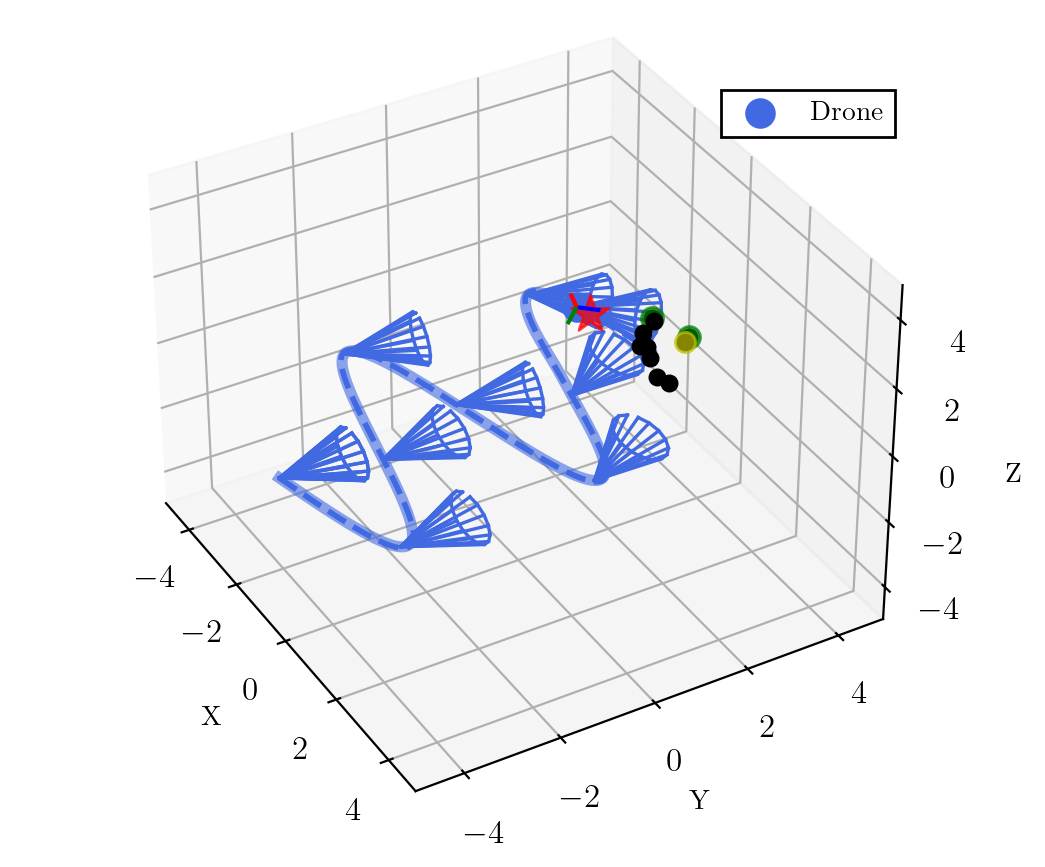
\includegraphics[width=7.5cm]{Fig/pcl_single_1.eps}\\
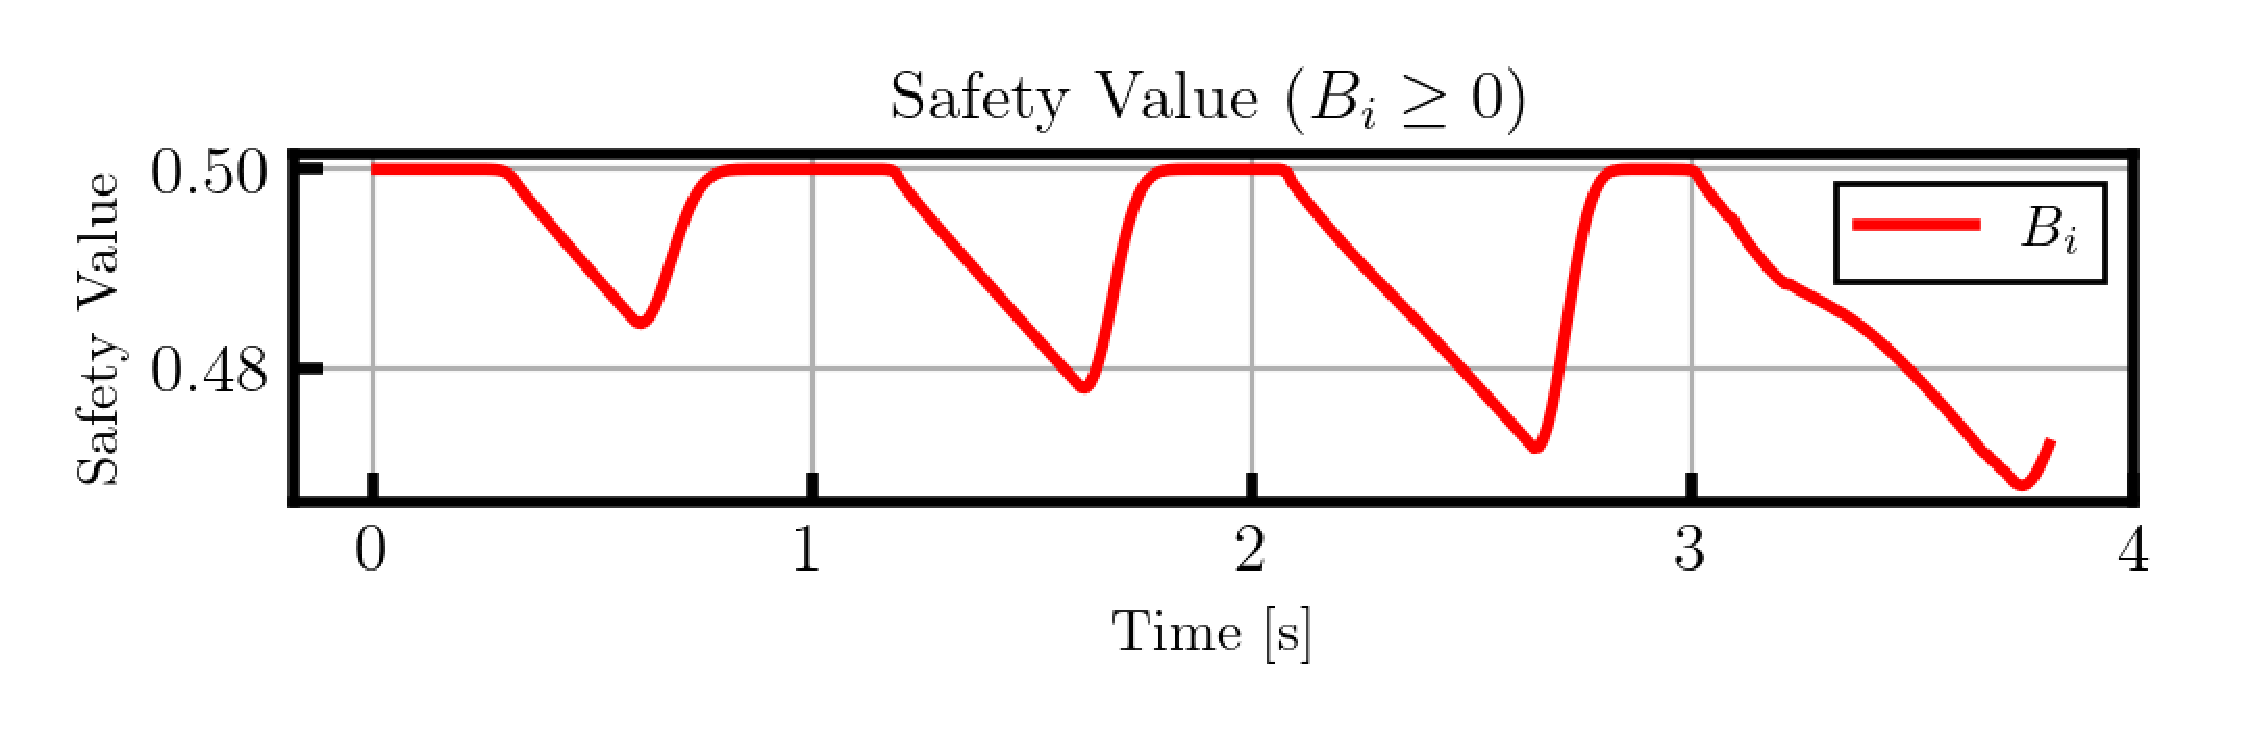
\includegraphics[width=8.0cm]{Fig/pcl_single_2.eps}\\
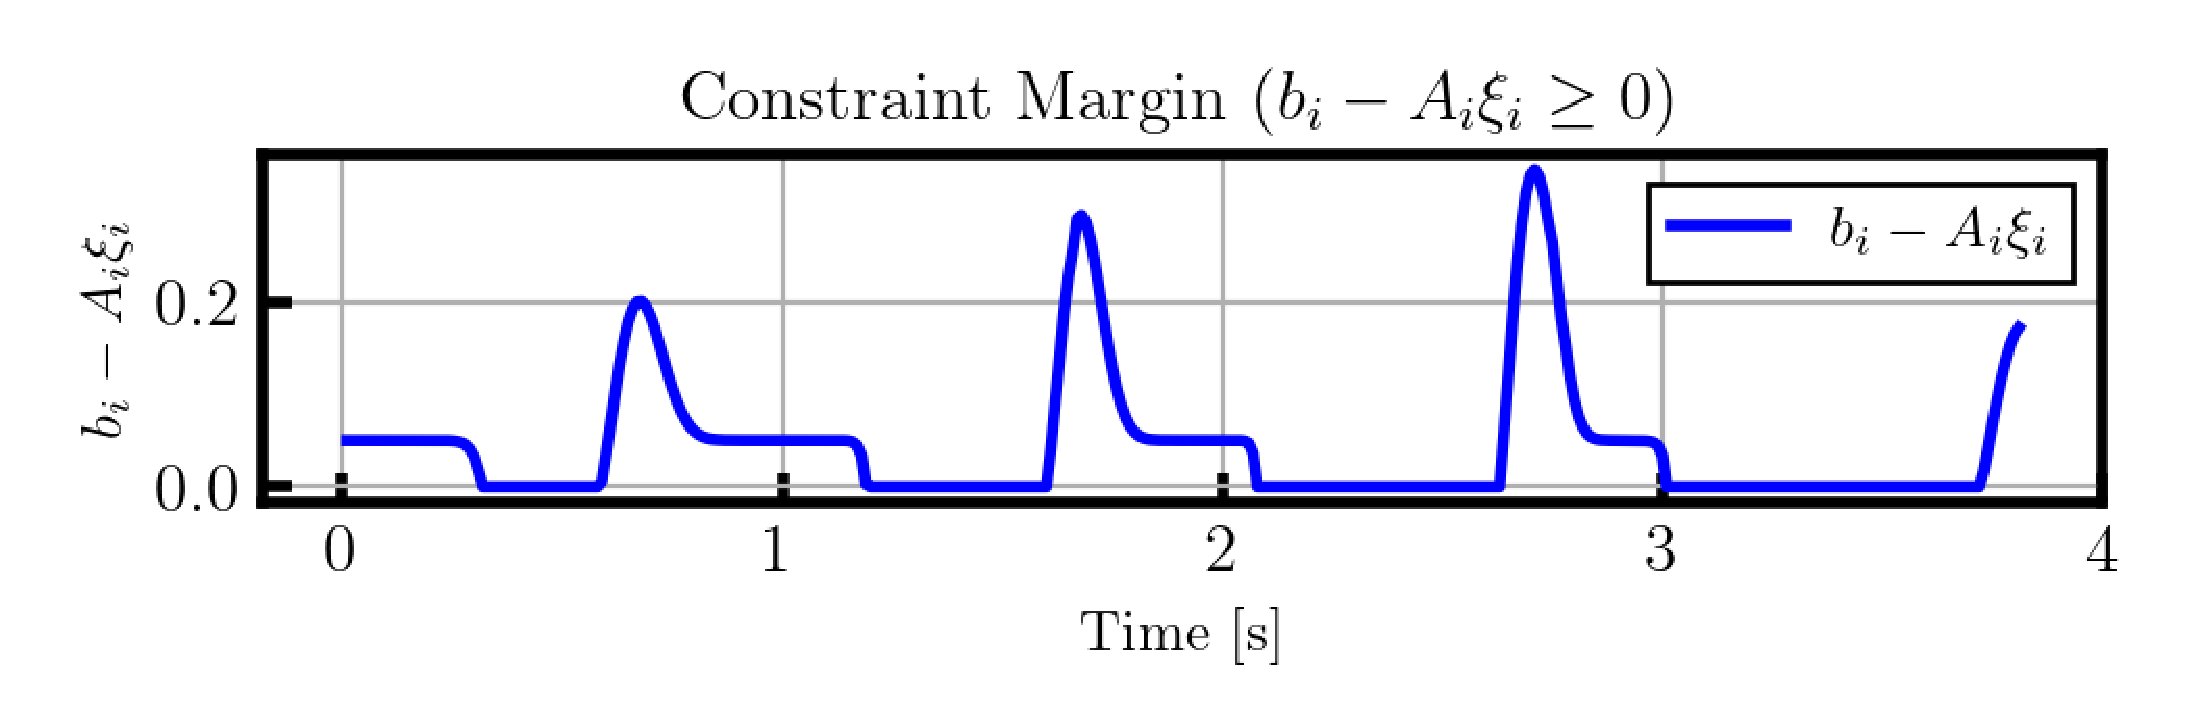
\includegraphics[width=8.0cm]{Fig/pcl_single_3.eps}
\caption{\label{fig:single_trajectory} Trajectory and view frustum of an agent tracking multiple feature points.}
\vspace{-4mm}
\end{center}
\end{figure}
For the simulation of an agent tracking multiple feature points, we used the same parameters as above, with the addition of probability constraint parameter $q = 0.5$ in \eqref{eq:multi_safe_set}.

Figure \ref{fig:single_trajectory} shows the trajectory and view frustum of an agent tracking multiple feature points. Similar to the single feature point case, the agent maintains multiple feature points within its field-of-view throughout the trajectory. The safety constraint $B_i$ remains positive, ensuring the forward invariance of the CBF.

\begin{figure}[h]
\begin{center}
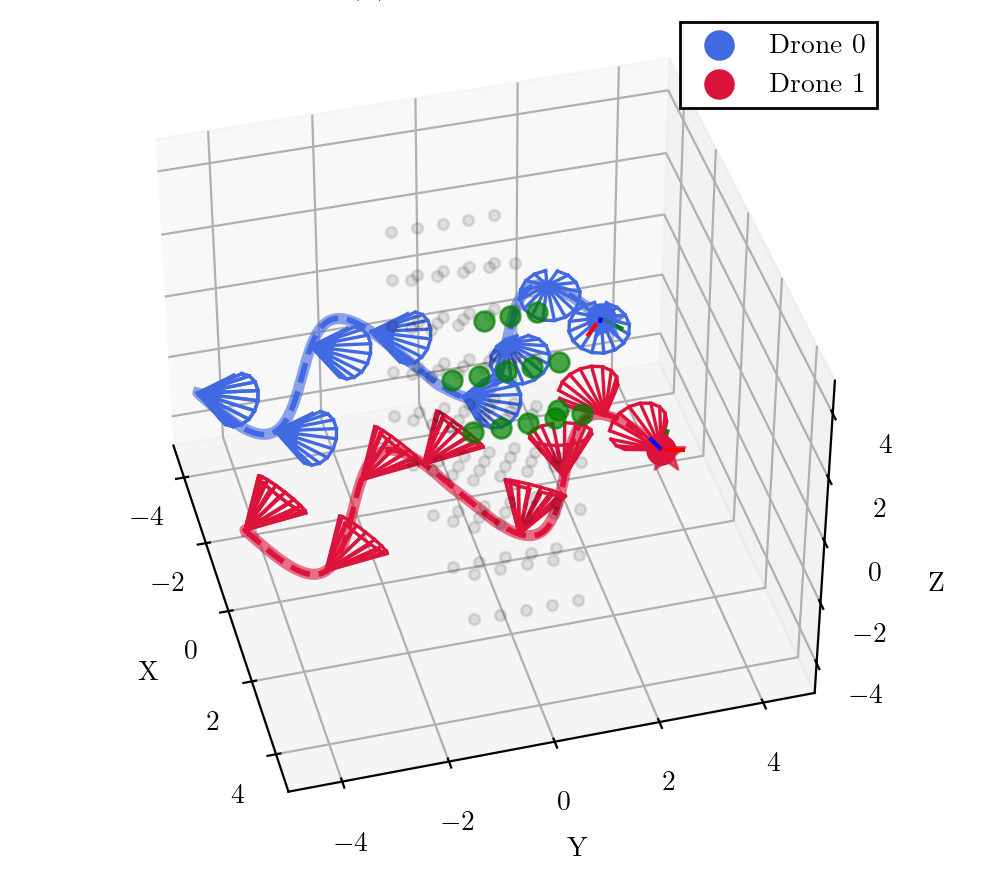
\includegraphics[width=7.5cm]{Fig/pcl_multi_centric_1.eps}\\
% \vspace{-2mm}
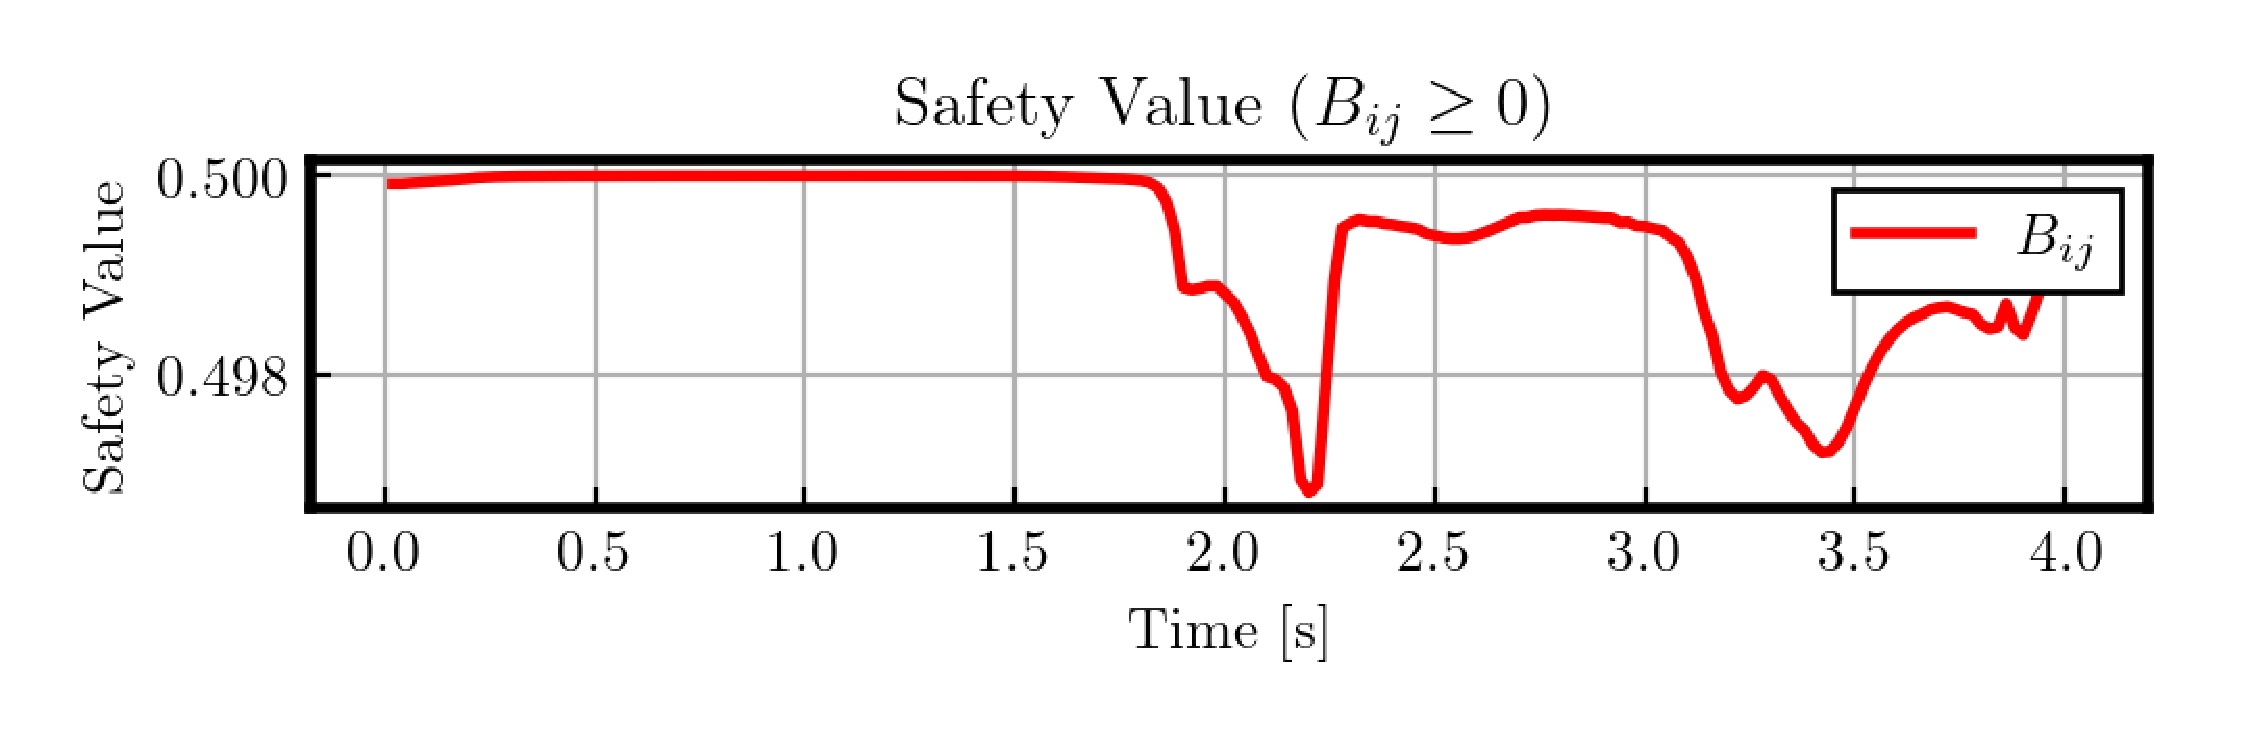
\includegraphics[width=8.0cm]{Fig/pcl_multi_centric_2.eps}\\
% \vspace{-2mm}
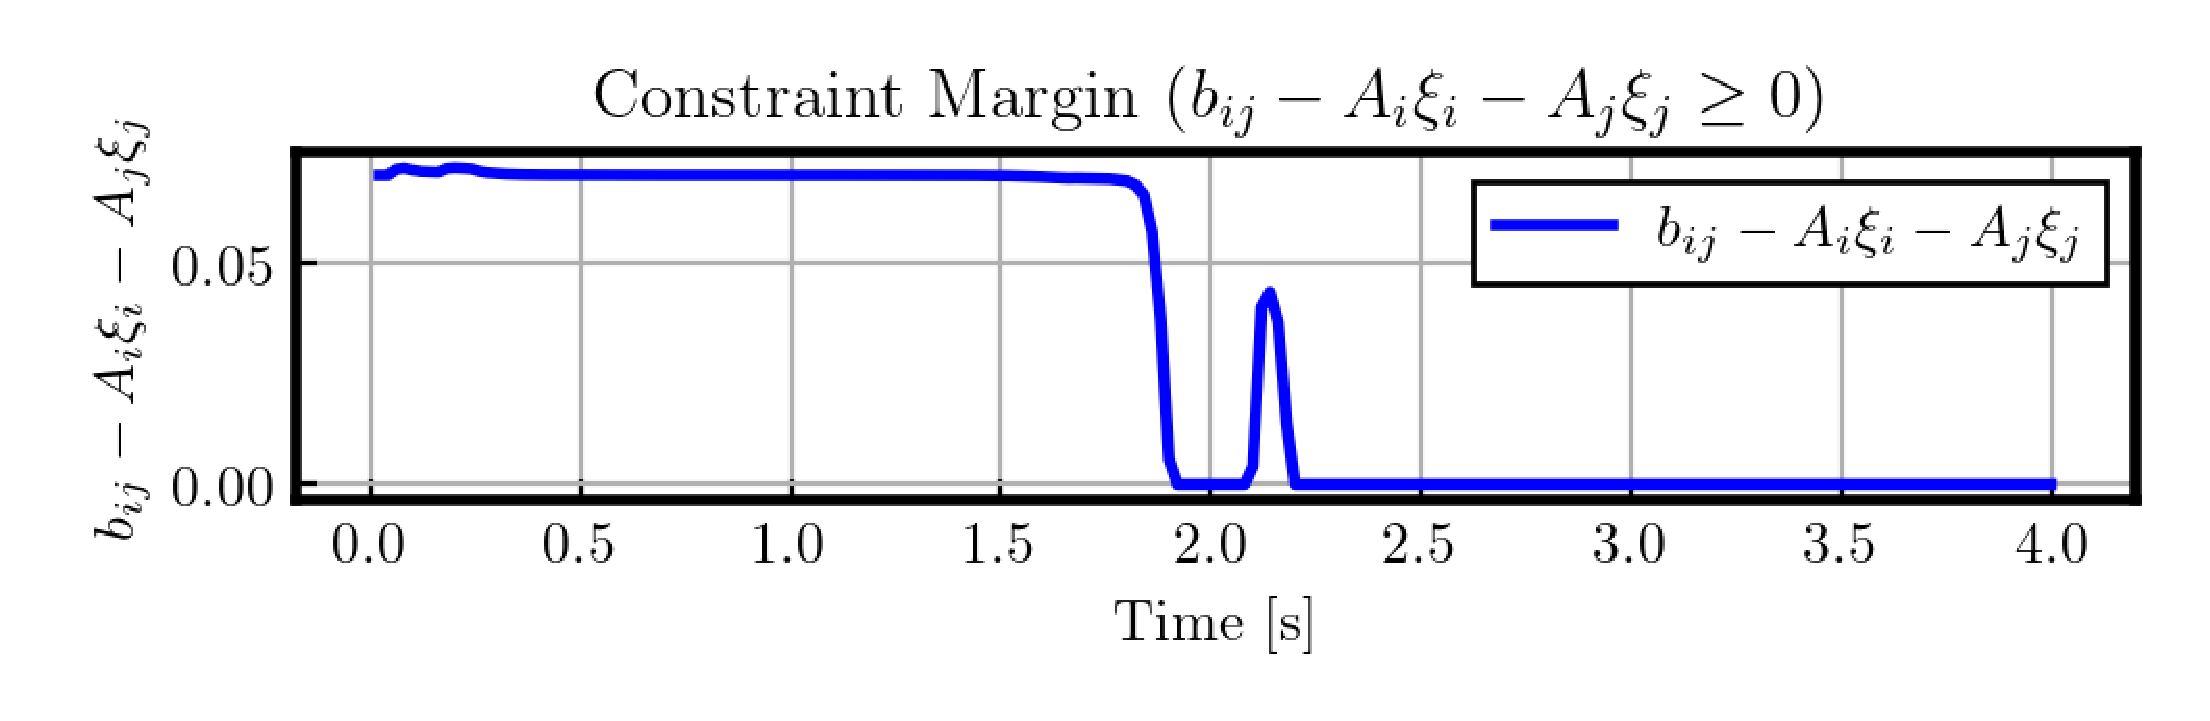
\includegraphics[width=8.0cm]{Fig/pcl_multi_centric_3.eps}
\caption{\label{fig:centralized_trajectory} Trajectories and view frustums of multiple agents in centralized control.}
\vspace{-4mm}
\end{center}
\end{figure}

For the centralized control simulation with multiple agents, we used the following parameters: sampling time $h = 0.02$, field-of-view angle $\Psi_{\mathcal{F}} = 30^{\circ}$, weight matrices $Q_1 = {\mathbf{I}}_3$ and $Q_2 = 0.0005 \times {\mathbf{I}}_6$, probability constraint parameter $q = 0.3$, and CBF class K function gain $\gamma_0 = 0.1$.

Figure \ref{fig:centralized_trajectory} shows the trajectories and view frustums of multiple agents in centralized control. The agents maintain shared feature points within their field-of-view throughout the trajectory. The safety constraint $B_{ij}$ remains positive, ensuring the forward invariance of the CBF.

\subsection{Distributed CBF}

For the distributed control simulation, we used the following parameters: sampling time $h = 0.02$, field-of-view angle $\Psi_{\mathcal{F}} = 30^{\circ}$, weight matrices $Q_1 = 0.5 \times {\mathbf{I}}_3$ and $Q_2 = 0.00001 \times {\mathbf{I}}_6$, probability constraint parameter $q = 0.3$, CBF class K function gain $\gamma_0 = 0.1$, and distributed optimization penalty parameter $c = 1.0$ in \eqref{eq:pdmm_algorithm}.

\begin{figure}[h]
\begin{center}
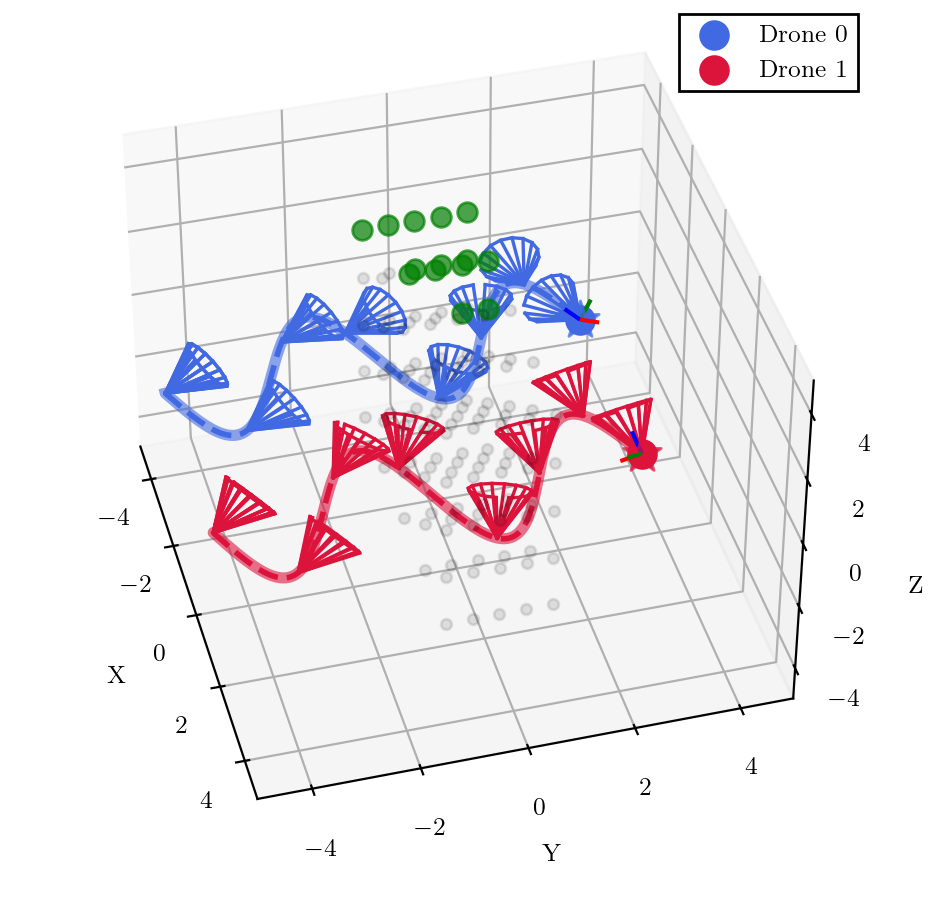
\includegraphics[width=7.0cm]{Fig/pcl_multi_distrib_1.eps}\\
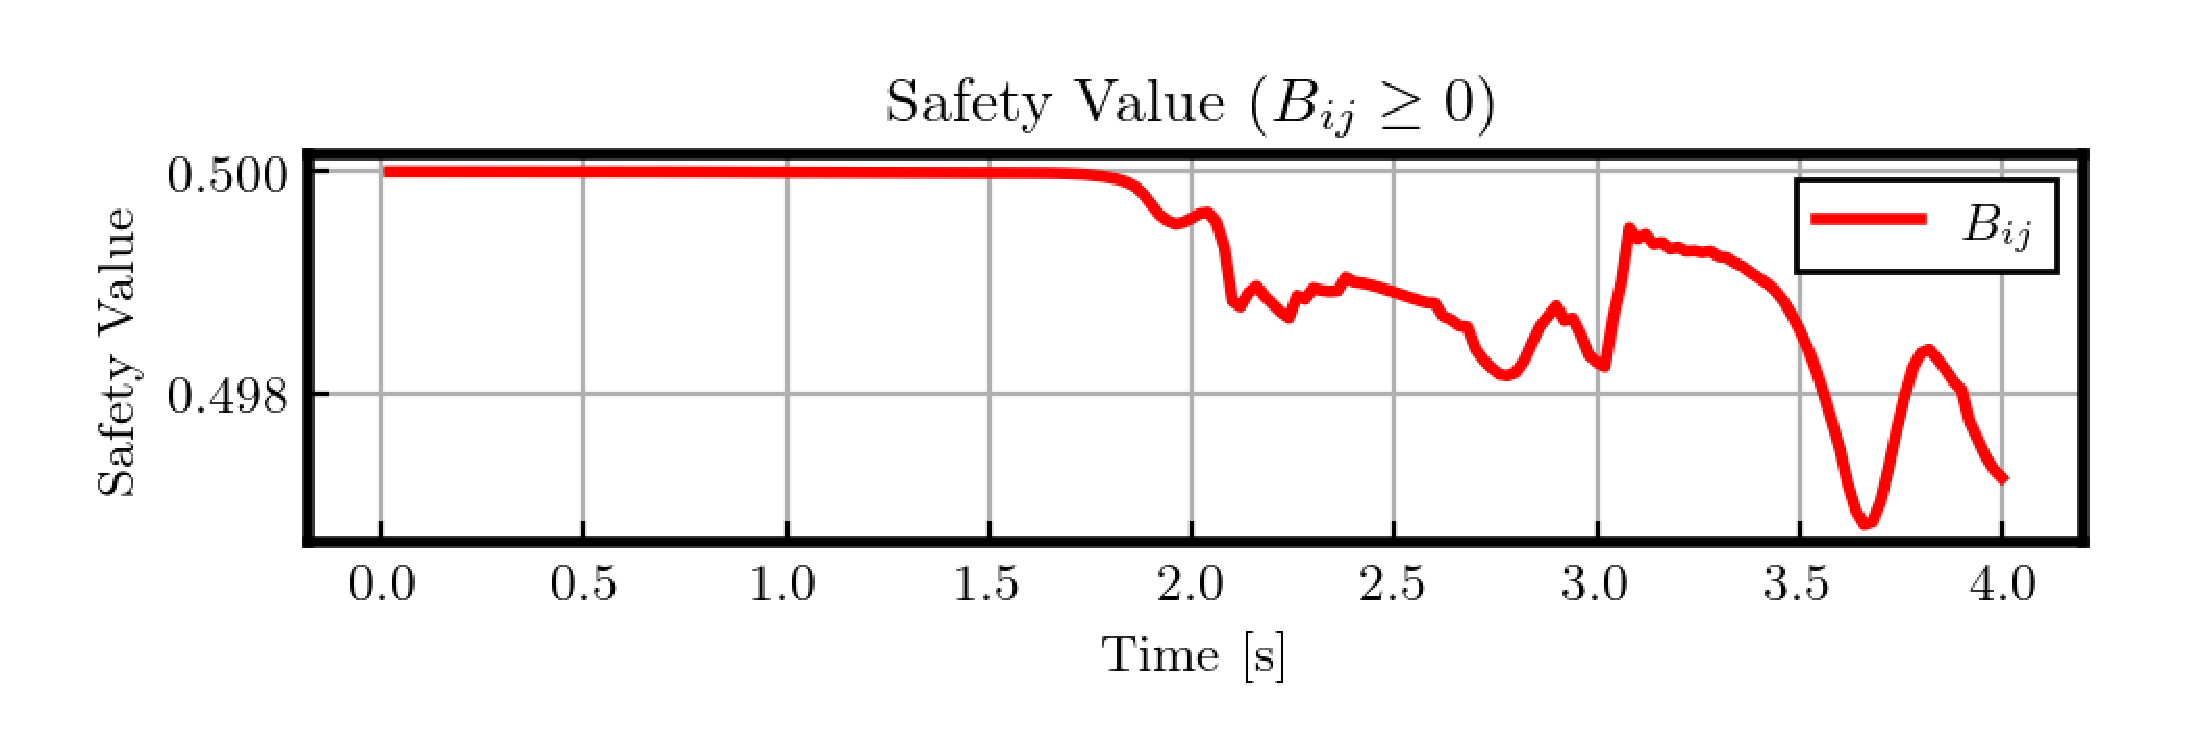
\includegraphics[width=8.0cm]{Fig/pcl_multi_distrib_2.eps}\\
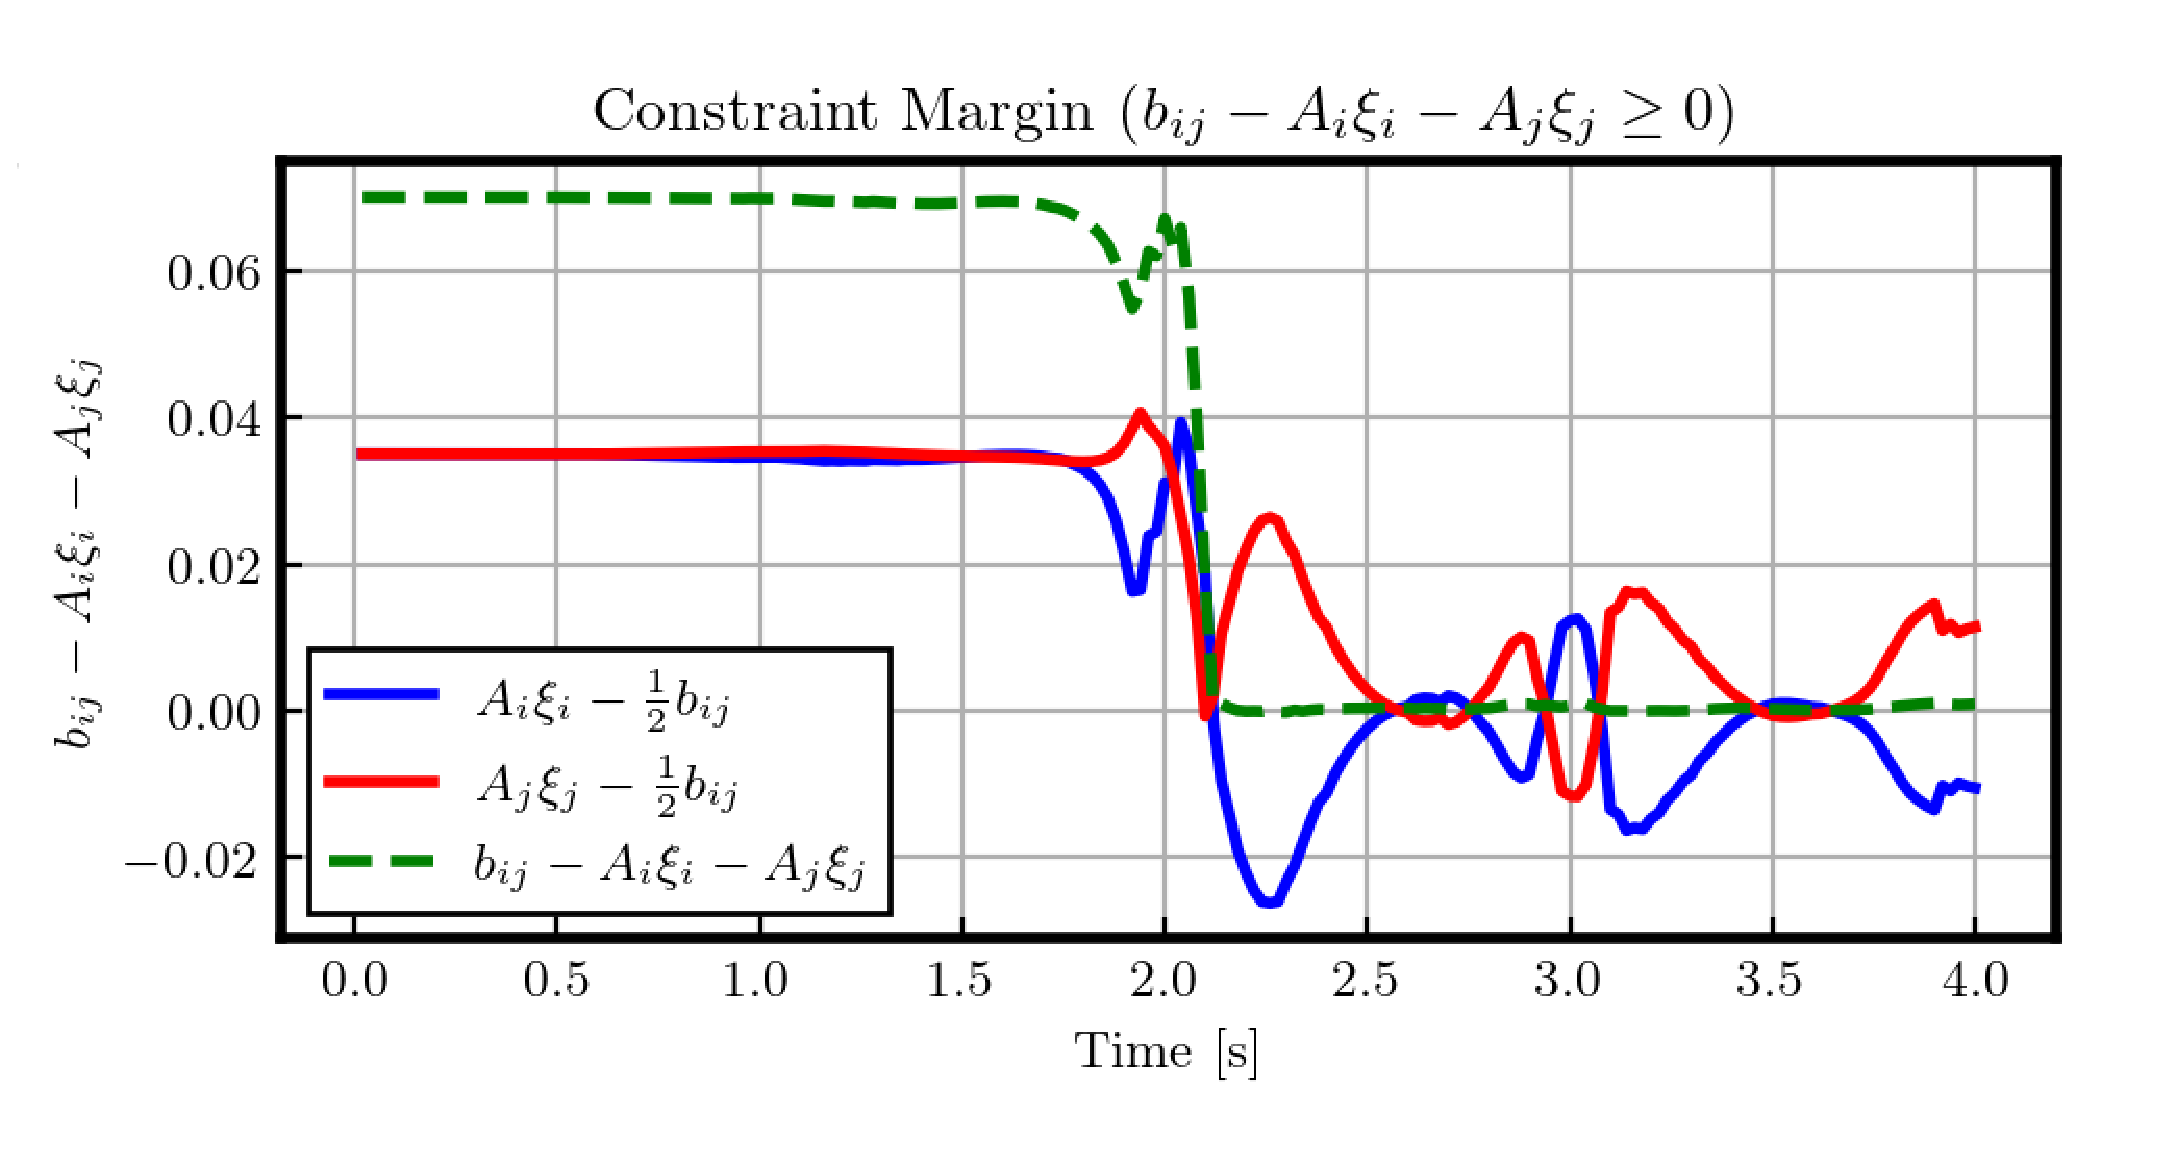
\includegraphics[width=8.0cm]{Fig/pcl_multi_distrib_3.eps}
\caption{\label{fig:distributed_trajectory} Trajectories and view frustums of multiple agents in distributed implementation.}
\vspace{-4mm}
\end{center}
\end{figure}
Figure \ref{fig:distributed_trajectory} shows the trajectories and view frustums of multiple agents in distributed implementation. The agents maintain shared feature points within their field-of-view throughout the trajectory. In distributed optimization, it is impossible to directly solve the original constraint equation, but the sum of $A_i\xi_i-\frac{1}{2}b_{ij}$ evaluated by agent $i$ and $A_j\xi_j-\frac{1}{2}b_{ij}$ evaluated by agent $j$ properly satisfies the constraint. This confirms that each agent can generate control inputs that satisfy global safety constraints using only local information.

These simulation results demonstrate that the proposed approach can generate control inputs that satisfy the field-of-view constraint for both single and multiple agents, in both centralized and distributed implementations.

\section{Conclusion}

This paper proposed a distributed control barrier function approach to guarantee field-of-view overlap for cooperative localization on SE(3). We introduced a probabilistic CBF that evaluates the visibility of feature points and incorporated it into a distributed optimization framework based on PDMM. The simulation results demonstrated the effectiveness of our approach in both centralized and distributed implementations.

Future work includes validating the approach on second-order and nonholonomic systems, as well as introducing probability functions based on covariance in self-localization. Specifically, we aim to design probability functions that directly bound the Cramer-Rao Lower Bound in maximum likelihood estimation, enabling the CBF to function as active perception for self-localization.

%%%%%%%%%%%%%%%% BIBLIOGRAPHY IN THE LaTeX file !!!!! %%%%%%%%%%%%%%%%%%%%%%
\begin{thebibliography}{9}
\bibitem{ref1}
D. Panagou, D. M. Stipanovic, and P. G. Voulgaris, ``Distributed dynamic coverage and avoidance control under anisotropic sensing,'' {\it IEEE Transactions on Control of Network Systems}, Vol. 4, No. 4, pp. 850-862, 2017.

\bibitem{ref2}
D. DeTone, T. Malisiewicz, and A. Rabinovich, ``SuperPoint: Self-supervised interest point detection and description,'' {\it Proceedings of the IEEE Conference on Computer Vision and Pattern Recognition Workshops}, pp. 224-236, 2018.

\bibitem{ref3}
R. Arandjelovic, P. Gronat, A. Torii, T. Pajdla, and J. Sivic, ``NetVLAD: CNN architecture for weakly supervised place recognition,'' {\it Proceedings of the IEEE Conference on Computer Vision and Pattern Recognition}, pp. 5297-5307, 2016.

\bibitem{ref4}
Z. Zhang, R. Tron, and S. Karaman, ``Distributed multi-robot formation control with communication delays and switching topologies,'' {\it IEEE Robotics and Automation Letters}, Vol. 7, No. 2, pp. 5182-5189, 2022.

\bibitem{ref5}
L. Sabattini, C. Secchi, and N. Chopra, ``Decentralized control for the maintenance of strong connectivity for directed graphs,'' {\it Proceedings of the Mediterranean Conference on Control and Automation}, pp. 978-986, 2013.

\bibitem{ref6}
A. D. Ames, X. Xu, J. W. Grizzle, P. Tabuada, ``Control barrier function based quadratic programs for safety critical systems,'' {\it IEEE Transactions on Automatic Control}, Vol. 62, No. 8, pp. 3861-3876, 2017.

% \bibitem{ref7}
% B. Capelli and L. Sabattini, ``Connectivity maintenance: Global and optimized approach through control barrier functions,'' {\it Proceedings of the IEEE International Conference on Robotics and Automation (ICRA)}, pp. 5590-5596, 2020.

\bibitem{ref7}
B. Trimarchi, F. Schiano, and R. Tron, ``A Control Barrier Function Candidate for Quadrotors with Limited Field of View,'' {\it arXiv:2410.01277 [eess.SY]}, 2025.

\bibitem{ref8}
D. Panagou and V. Kumar, ``Maintaining visibility for leader-follower formations in obstacle environments,'' {\it Proceedings of the IEEE International Conference on Robotics and Automation (ICRA)}, pp. 1811-1816, 2012.

\bibitem{ref9}
D. Dias, P. U. Lima, and A. Martinoli, ``Distributed Formation Control of Quadrotors under Limited Sensor Field of View,'' {\it Proceedings of the International Conference on Autonomous Agents and Multiagent Systems (AAMAS)}, pp. 1087-1095, 2016.

\bibitem{ref10}
R. Heusdens and G. Zhang, ``Distributed Optimisation With Linear Equality and Inequality Constraints Using PDMM,'' {\it IEEE Transactions on Signal and Information Processing over Networks}, Vol. 10, pp. 294-306, 2024.

\end{thebibliography}
\end{document}
